

\newcommand{\escaladefault}{0.85}

Incluimos un WBS híbrido de procesos y productos, para ilustrar los subcomponentes del proyecto. En la primera capa de este WBS se divide al sistema principal en subsistemas menores, cada uno de estos encargado de una tarea en particular.
Se describen también los procesos necesarios para poder desarrollar con éxito estos subsistemas. Además 
de los subsistemas, algunos subproductos como documentaciones y modulos auxiliares necesarios para el desarrollo 
de un sistema respectivo fueron declarados.
Es esperable que los procesos declarados dentro de este diagrama, conforme avance el proyecto, sean sintetizados en tareas 
a realizar en alguna iteración en particular.

El WBS define dependencias tentativas en el proyecto, sin embargo, estas estan sujetas a cambios y es esperable que deban 
ajustarse a lo largo del proyecto.

Vale destacar que para el desarrollo de ciertos productos, de los cuales esperamos que esten sujetos a cambios, se tuvo en 
cuenta un proceso de "correcion de requerimientos".

\begin{figure}[H]
\centering
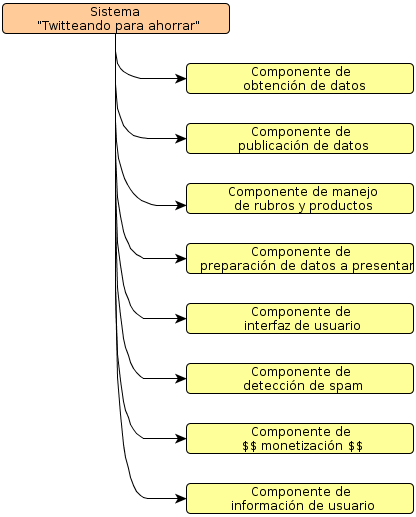
\includegraphics[scale=\escaladefault]{graficos/wbs/primera_capa.png}
\caption{Vista general del WBS: componentes del proyecto}
\end{figure}

\begin{figure}[H]
\centering
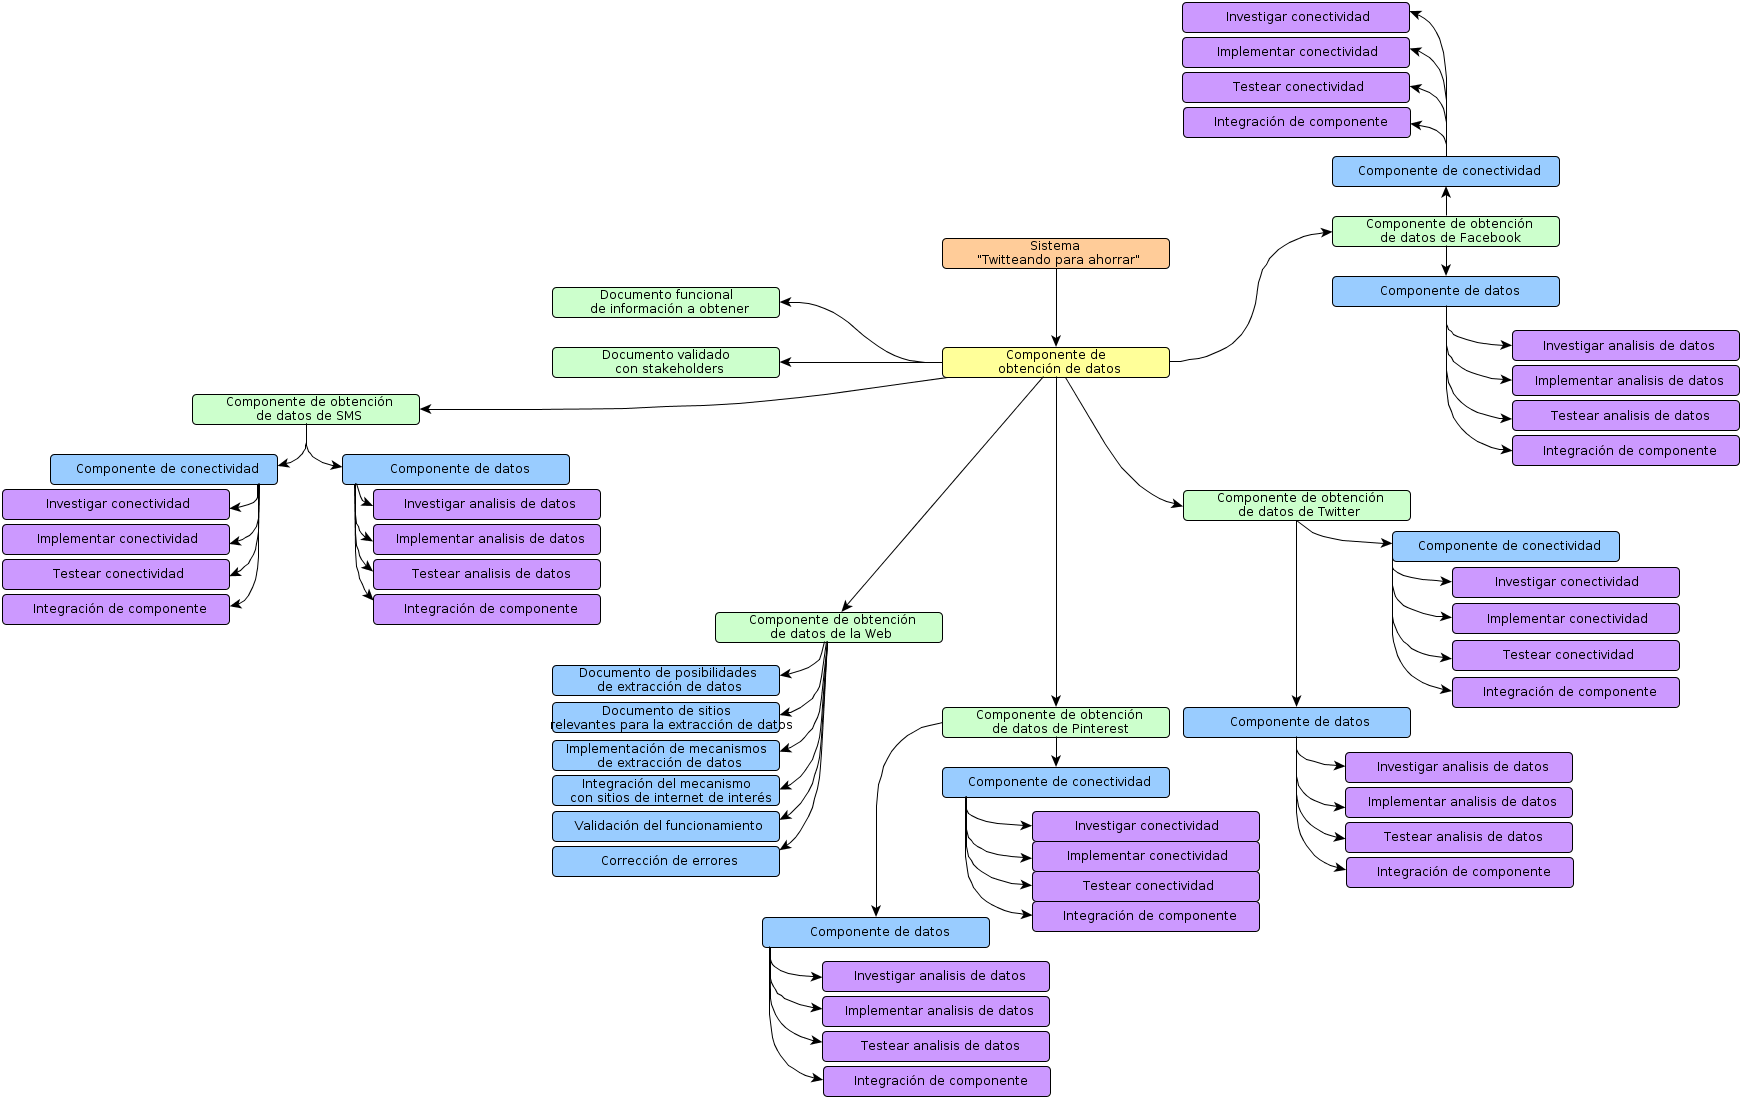
\includegraphics[scale=\escaladefault]{graficos/wbs/comp_obtencion_datos.png}
\caption{Componente de obtención de datos}
\end{figure}

\begin{figure}[H]
\centering
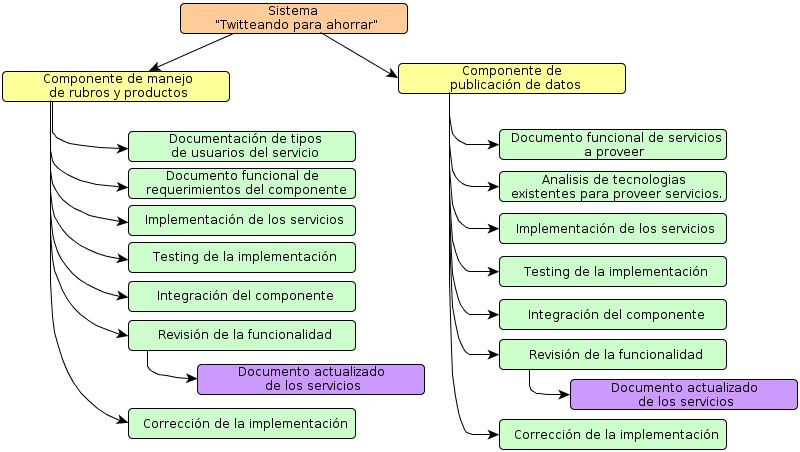
\includegraphics[scale=\escaladefault]{graficos/wbs/comp_rubros_y_api.png}
\caption{Componente de publicación de datos y componente de rubros y productos}
\end{figure}

\begin{figure}[H]
\centering
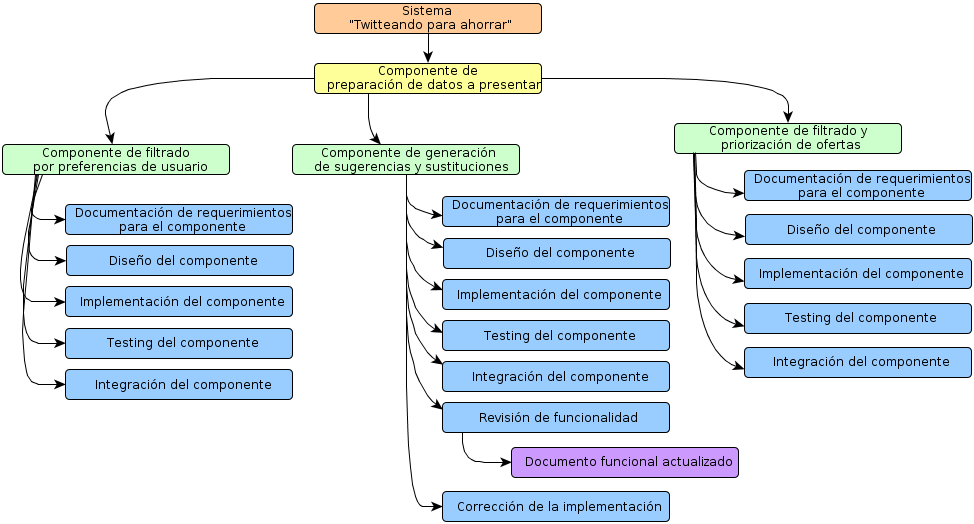
\includegraphics[width=\textwidth]{graficos/wbs/com_prep_de_datos.png}
\caption{Componente de preparación de datos a presentar}
\end{figure}

\begin{figure}[H]
\centering
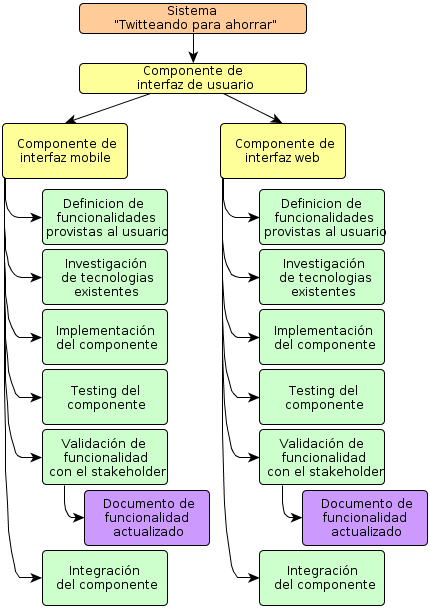
\includegraphics[scale=\escaladefault]{graficos/wbs/comp_interfaz.png}
\caption{Componente de interfaz de usuario}
\end{figure}

\begin{figure}[H]
\centering
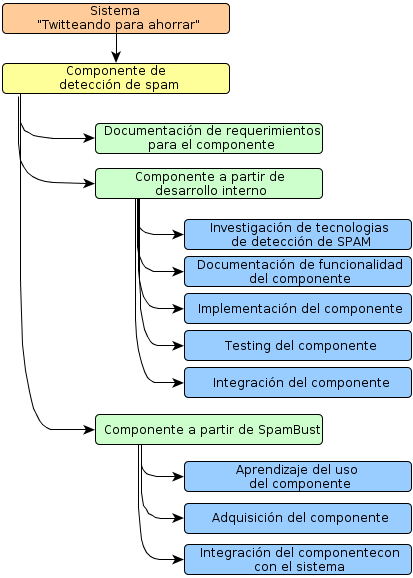
\includegraphics[scale=\escaladefault]{graficos/wbs/comp_de_spam.png}
\caption{Componente de detección de spam}
\end{figure}

\begin{figure}[H]
\centering
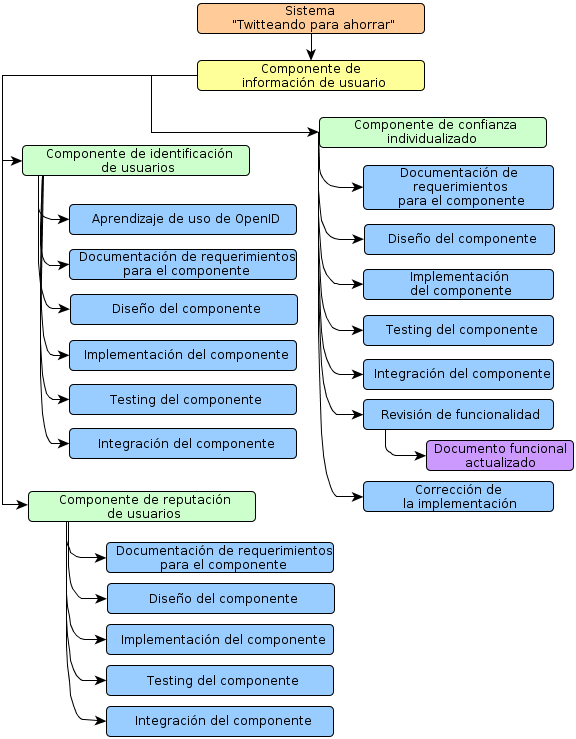
\includegraphics[scale=\escaladefault]{graficos/wbs/comp_de_info_de_usuario.png}
\caption{Componente de información de usuario}
\end{figure}

\begin{figure}[H]
\centering
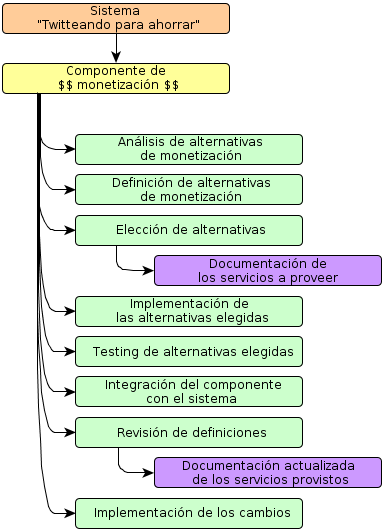
\includegraphics[scale=\escaladefault]{graficos/wbs/comp_monetizacion.png}
\caption{Componente de monetización}
\end{figure}

